\subsection{Leistung und Verluste \hfill IP}
\begin{footnotesize}
    \begin{empheq}[box=\fbox]{align*}
        P_{\text{mech}} &= P_{el} - p_{el, \text{Verl}} = U \cdot (I-I_0) - R\cdot I \cdot (I-I_0)
        \\ &= -R \cdot I^2 + (U+R\cdot I_0)\cdot I - U\cdot I_0
        \\ P_{\text{mech, max}} &= \frac{R}{4} \cdot \left(\frac{U_N}{R} - I_0\right)^2 \quad \mid \quad P_{el} = U \cdot I
    \end{empheq}
    \begin{empheq}[box=\fbox]{align*}
                P_{\text{mech, } \eta \text{max}}  &=
            \begin{cases}
            2\pi \cdot M_{\eta, \text{max}}\\ 
            2\pi \cdot M_{\eta, \text{max}} \cdot \left(n_0 - \frac{n_0 \cdot M_{\eta, \text{max}}}{M_H}\right)\\
            \eta_{\text{max}} \cdot P_{an} = \eta_{\text{max}} \cdot n \cdot I_{\eta, \text{max}}\\
            -R \cdot I_{\eta, \text{max}}^2 + (n + R\cdot I_0) \cdot I_{\eta, \text{max}} - n \cdot I_0\\
            \end{cases} 
            \\
            n  &=
            \begin{cases}
            k_n \cdot U\\
            k_n \cdot U - \frac{k_n}{k_M} \cdot R \cdot M \quad \quad (\text{R berücksichtigt})\\
            n_0 - \frac{n_0}{M_H} \cdot M \quad \quad (\text{lineare Drehzahlkennlinie})\\
            \end{cases}
            \\n_0 = k_n \cdot &(U_N - I_0\cdot R) \quad \mid \quad U = R\cdot I \quad \mid \quad I_0 = \frac{M_R}{k_M}
            \\I_{\eta, \text{max}} &= \frac{M_{\eta, \text{max}} + M_R}{k_m} \quad \mid \quad k_n = \frac{1}{2\pi} \cdot \frac{1}{k_M}
            \\M &= k_M \cdot I \quad \mid \quad M_R = k_M \cdot I_0 
            \\M_H = &\frac{n_0}{k_n} \cdot \frac{k_M}{R} \text{ für } U_N \quad \mid \quad M_{\text{mech, max}} = \frac{M_H - M_R}{2}
            \\M_{\eta, \text{max}} &= \sqrt{M_H \cdot M_R} \quad \mid \quad \eta_{\text{max}} = \left(1 - \sqrt{\frac{I_0 \cdot R}{U_N}}\right)^2
            \\ \eta &= \frac{-R \cdot I^2 + (U+RI_0) \cdot I - UI_0}{U \cdot I}
    \end{empheq}
    \begin{empheq}[box=\fbox]{align*}
        [W] &= [V] \cdot [A] = \left[ \frac{Nm}{s}\right] \quad \mid \quad [A] = \frac{[W]}{[V]} = \frac{[Nm]}{[V]}
        \\ [V] &= \frac{[W]}{[A]} = \left[\frac{Nm}{A\cdot s}\right] = \left[\frac{kg \cdot m^2}{A\cdot s^2}\right] \quad \mid \quad [\Omega] = \left[\frac{V}{A}\right]
        \\ [V \cdot min] &= 60'000 \left[\frac{mNm}{A}\right]
    \end{empheq}
    $R$ = Widerstand; $U_N$ = Nennspannung, $I_0$ = Leerlaufstrom

    \cbreak

    \centering{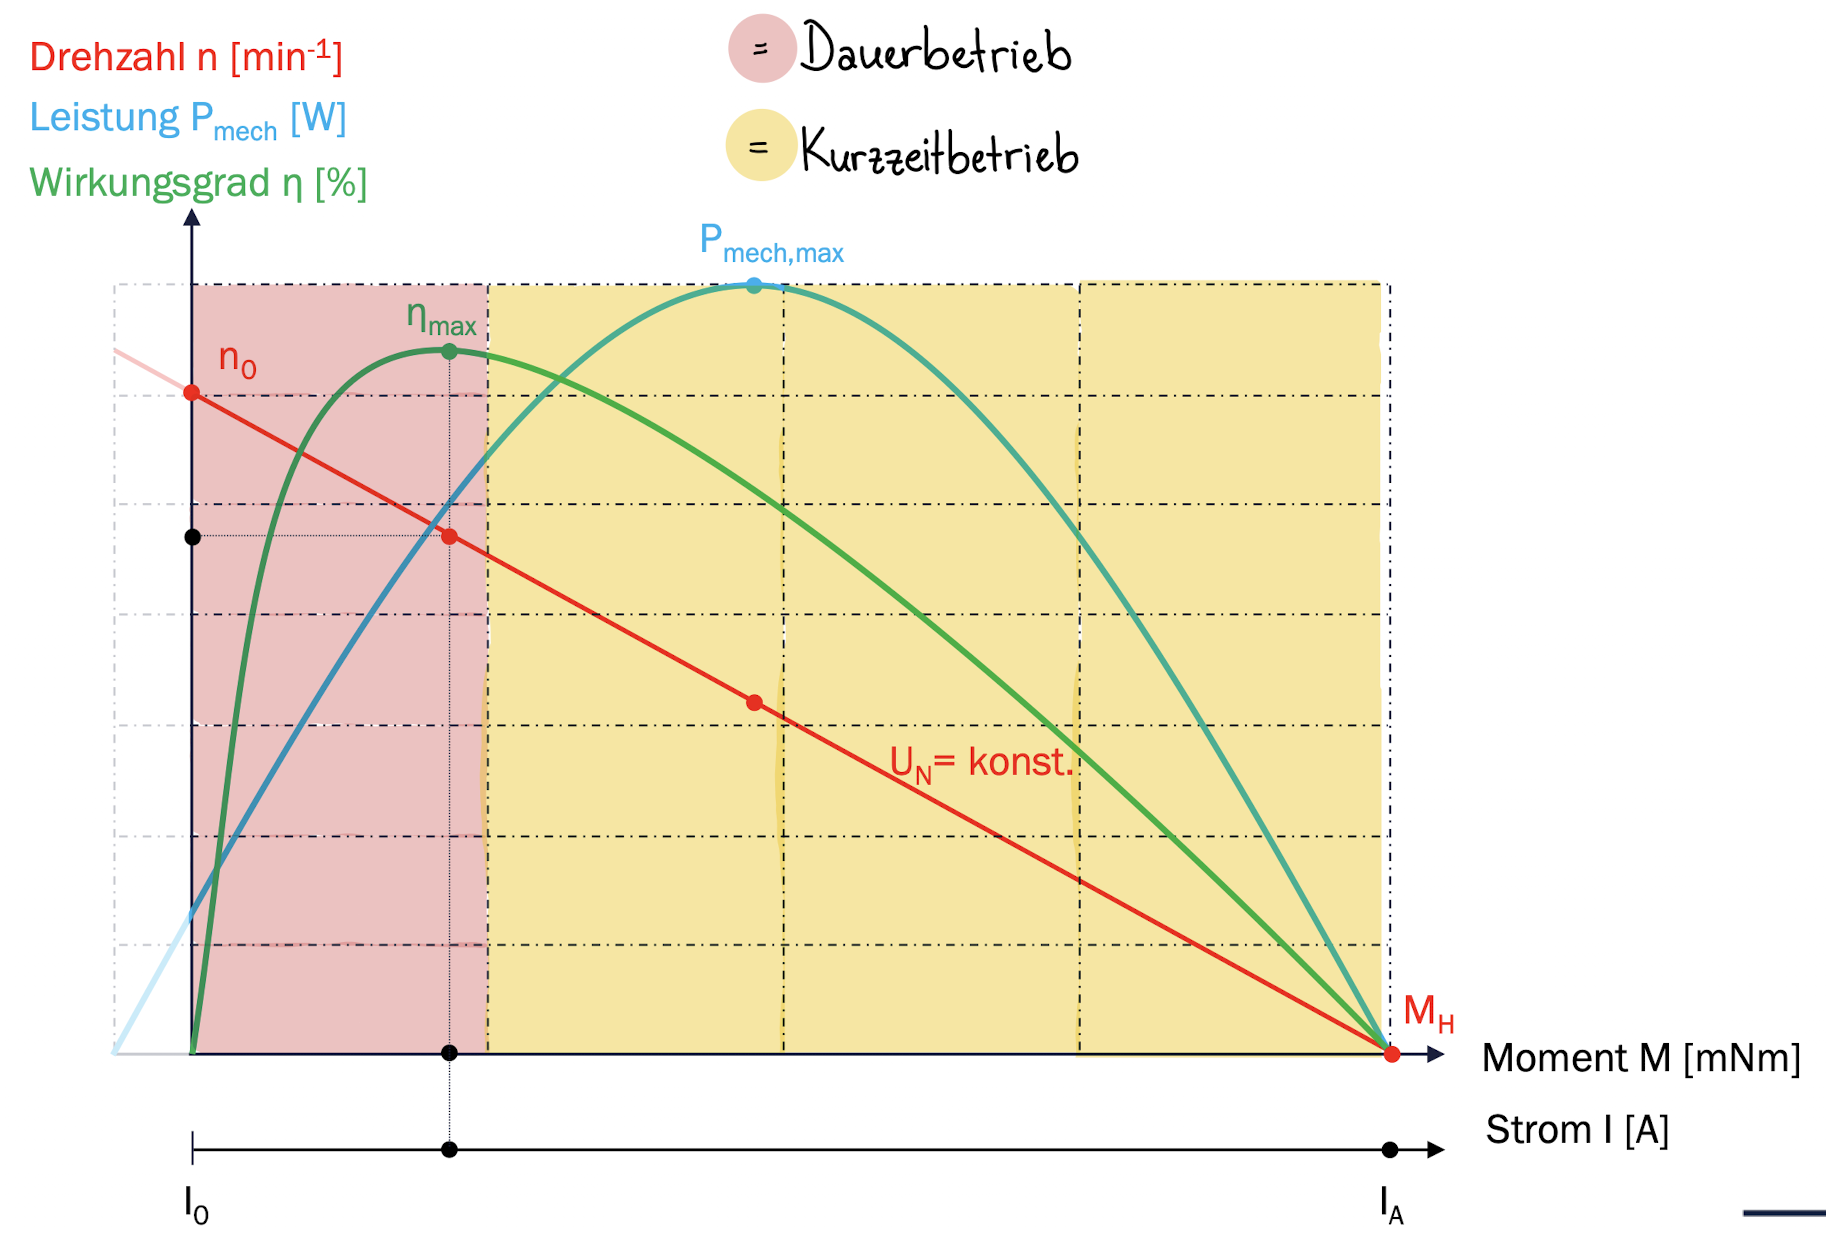
\includegraphics[width = 1.0\linewidth]{MAEIP_Motorkennlinien}}
\end{footnotesize}